\documentclass[13pt]{article}
\usepackage{graphicx}

\begin{document}

\title{Project 2 Report}
\author{M Shepherd, 19059020@sun.ac.za \\ M von Fintel, 20058837@sun.ac.za}
\date{22 August 2018}

\maketitle

\centerline{Reliable Blast User Datagram Protocol (RBUDP)}

\newpage

\section{Introduction}

It was required for this project to send files over a network using the Reliable
Blast User Datagram Protocol (RBUDP). The Transmission Control Protocol (TCP) was
also implemented for comparison with RBUDP. The project was implemented in Java
using Java Sockets.
\\\\
The project consists of a Sender and a Receiver. The following report details
what they respectively do, what features have been implemented, how they have been
implemented, how the project is run and how it was tested.

\section{Project Overview}

\subsection{The Sender}

When the Sender is run, a pane starts with a few buttons and a text area.
A \texttt{ServerSocket} is made over port 8000 and the Sender allows a Receiver to connect.
A \texttt{PrintStream} is made for communication between the Sender and the Receiver.
When the "Open File to Send" button is clicked, a \texttt{JFileChoser} window starts, which
allows the user to select a file from the user's filesystem. Now the two send
buttons are enabled, one for sending via TCP and the other for sending via RBUDP.
\\\\
If the user chooses to send the file via TCP, the Sender first checks that there
is a Receiver connected. If one is connected, \texttt{FileInputStream} and
 \texttt{BufferedInputStream}'s are then used to read in 65000 byte portions of the
data from the file selected into a \texttt{byte} array. These \texttt{byte} arrays
are then sent to the Receiver, where they are pieced together.
\\\\
If the user chooses to send the file via RBUDP, the Sender first checks that there
is a Receiver connected. If one is connected, \texttt{FileInputStream} and
 \texttt{BufferedInputStream}'s are then used to read in 65000 byte portions of the
data from the file selected into a \texttt{byte} array. This number was chosen, as
it was the larges number that the network would allowand our sequence ID is 50 bytes.
These \texttt{byte} arrays are then added into a \texttt{LinkedList} of type
\texttt{DatagramPacket}. Then the Sender iterates through the \texttt{LinkedList}
and sends each datagram packet via a \texttt{DatagramSocket}.

\subsection{The Receiver}

When the Receiver is run, the user is prompted to enter the host they wish to
connect to. If they input a valid host, the Receiver connects to that host and is
ready to receive files from the Sender. The Receiver waits until the Sender
sends a file.
\\\\
If a file is sent via TCP, it is read into the output file using a
\texttt{FileOuputStream} and a \texttt{BufferedOutputStream}. Then the Receiver thread
is closed. A new thread is then made in preparation for the next incoming file,
whether one follows or not. The progress bar is updated with the progress of the
incoming file. Output is printed to the text area to keep the user informed of
certain events.
\\\\
If a file is sent via RBUDP, a method that listens for datagram packets is called.
A \texttt{byte LinkedList} is populated with all ID's of the expected packets.
All the received packets are also added to a \texttt{LinkedList}. The progress bar
is updated with the progress of the incoming packets compared to the total filesize.
The received packets are then compared to the expected packets and the packets that got lost
are then determined. The received packets are read into the output file using a
\texttt{FileOuputStream} and a \texttt{BufferedOutputStream}. Then the Receiver thread
is closed. A new thread is then made in preparation for the next incoming file,
whether one follows or not. Output is printed to the text area to keep the user informed of
certain events.

\section{Features}

\subsection{Extra Features}

For your relaxation, the RBUDP is really slow. This enables you to take some time
to go and get a coffee.

\subsection{Unimplemented Features}

All features were implemented.

\section{Description of Source Files}

Our project consists of two files, namely \texttt{SenderPane.java} and
\texttt{RecieverPane.java}.
\\\\
\texttt{SenderPane.java} contains all the code for the Sender. This includes the
code that sets up the GUI, the code that makes the \texttt{Socket} connections
and the code that sends via TCP and RBUDP.
\\\\
\texttt{RecieverPane.java} contains all the code for the Receiver. This includes the
code that sets up the GUI, the code that connects to the Sender and the code that
receives the files sent via TCP and RBUDP.

\section{Program Flow Description}

For instructions on how to compile and run, please see the Compilation and Execution
section.
\\\\
Once the Sender and Receiver is running and the user on the receiving side has
entered the IP address of the Sender, the program creates the connection. Then,
the user on the Sender side presses the "Open File to Send". A \texttt{JFileChoser}
opens and the user can select a file from their filesystem. Then the user is presented
with two options, to send via TCP or RBUDP. For a detailed description of both of
these processes, please the Project Overview section of this report. The Receiver
receives the files and saves them to the user on the receiver side's filesystem.
The Receiver then restarts and waits to see if another file is sent.

\section{Experiments and Testing}

To test how the project responded to sending different filesizes, an experiment
was performed. Files, with sizes ranging from one megabyte to one gigabyte,
were sent via the protocols to test how they scale. We also used iptables to
increase the chance of packet loss in order to test how the protocols dealt with
the loss of packets. Finally, we tested the protocols with varying packet sizes to 
better understand what made the different protocols run faster.

\subsection{Incrementing File Sizes}

\begin{table}[h!]
\caption{Incrementing File Sizes with Zero Packet Loss}
\begin{center}
\begin{tabular}{|c|c|c|c|c|}
\hline RBUDP(s) & RBUDP (mb/s) & TCP (mb/s) & TCP(s) & File Size (mb) \\
\hline 0.299  &3.34&50.00&0.020&1 \\
\hline 36.288 &2.76&77.70&1.487&100 \\
\hline 71.811 &2.79&66.40&3.012&200 \\
\hline 106.142&2.83&68.93&4.352&300 \\
\hline 144.243&2.77&67.77&5.902&400 \\
\hline 179.734&2.78&69.06&7.240&500 \\
\hline 216.174&2.78&68.21&8.796&600 \\
\hline 250.166&2.80&62.25&11.245&700 \\
\hline 287.366&2.78&65.36&12.240&800 \\
\hline 321.540&2.80&65.59&13.721&900 \\
\hline 359.550&2.78&62.00&16.130&1000 \\
\hline
\end{tabular}
\end{center}
\end{table}

\begin{figure}[h!]
  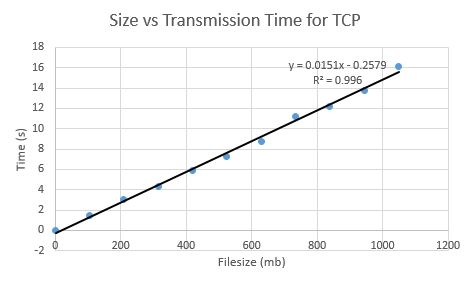
\includegraphics{1m-1gTCP.JPG}
  \caption{A comparison of transmission times and filesize for TCP}
\end{figure}

\begin{figure}[h!]
  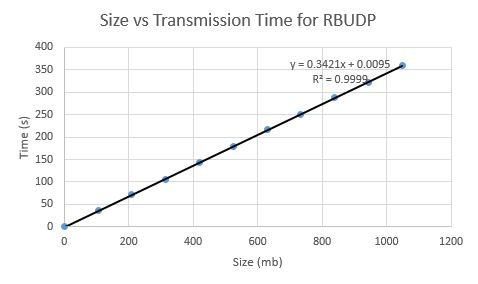
\includegraphics{1m-1gRBUDP.JPG}
  \caption{A comparison of transmission times and filesize for RBUDP}
\end{figure}

In both of the graphs below, the correlation coefficient is almost exactly one. This
shows that between one Gigabyte and one Megabyte, both of these protocols do
scale almost perfectly.

\clearpage

\subsection{Incrementing Packet Size}

For RBUDP, increasing the packet size ad a massive affect on the transmission
speed of the 50 b file. This shows that pushing the packet size to its upper
limit of allowed transmission size will allow data to be transmitted more
efficiently. For TCP, however, the packet size had little, to no affect on the
transmission speed, given how high the speed was originally.

\begin{table}[!h]
\caption{Incrementing Packet Size with Zero Packet Loss and 50mb file}
\begin{center}
\begin{tabular}{|c|c|c|c|c|}
\hline RBUDP(s) & RBUDP (mb/s) & TCP(s) & TCP (mb/s) & Packet Size (b) \\
\hline 104.979& 0.47 & 0.066&757.6&10000 \\
\hline 52.570 & 0.96 & 0.067&746.2&20000 \\
\hline 34.902 & 1.43 & 0.059&847.5&30000 \\
\hline 26.175 & 1.91 & 0.060&833.3&40000 \\
\hline 20.974 & 2.38 & 0.057&877.2&50000 \\
\hline 17.454 & 2.87 & 0.057&877.2&60000 \\
\hline 16.089 & 3.11 & 0.058&862.1&65000 \\
\hline
\end{tabular}
\end{center}
\end{table}

\begin{figure}[!h]
  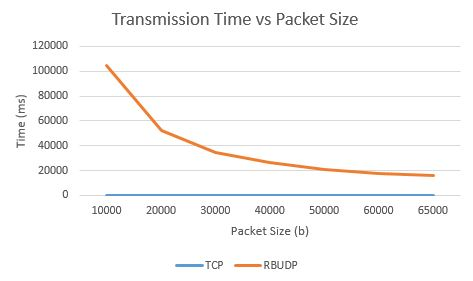
\includegraphics{packetSize.JPG}
  \caption{A comparison transimission times vs packet size with RBUDP and TCP}
\end{figure}

\subsection{Constant Packet Loss and File Size}

\begin{table}
\caption{10$\%$ Packet Loss Enforced with 50mb file}
\begin{center}
\begin{tabular}{|c|c|c|c|c|}
\hline RBUDP(ms) & RBUDP (mb/s) & RBUDP Packet Loss \% & TCP(ms) & TCP (mb/s) \\
\hline 17.464 &2.86&0   &0.058 & 862.1 \\
\hline 66.859 &0.75&8.39&2.612 & 19.142\\
\hline 71.012 &0.70&9.05&2.134 & 23.43 \\
\hline 72.234 &0.69&11  &3.508 & 14.243\\
\hline 67.682 &0.74&9.1 &3.799 & 13.161\\
\hline 60.564 &0.83&10.1&3.789 & 13.196\\
\hline
\end{tabular}
\end{center}
\end{table}

In this table above, we can clearly see that with an almost constant packet loss
enforced with iptables, the transmission times of a 50mb file more closely
resemble the unhindered transmission times of a 200mb file for both protocols.
This shows that both protocols are affected equally by packet loss.

\section{Issues Encountered}

\subsection{Unique Sequence Numbers}

Most of the issues that we encountered were involving the transmission and
parsing of the unique identifiers and most of these issues were solved with a
small amount of research into how Java deals with byte arrays and strings.
\\\\
This first issue that was encountered was that the byte arrays that were sent
were not appearing to be the same as the received arrays. This turned out to be
an issue with how we were converting them into String values for comparison in
the receiver. This was solved by learning that the \texttt{toString} method for
Java \texttt{arrays} returns the array type and memory address, while creating a
new string, using the byte array as an argument returns the needed String.
\\\\
The second issue that we encountered was that when converting a byte array to a
String, and then back to a byte array, the byte arrays would not be consistent
in size. This issue was solved by taking the size of the byte array into
consideration when being sent and received with the sockets.

\subsection{Design Issues}

The last significant issue that we encountered was dues to design errors. Our
RBUDP algorithm was initially not created to deal with lost or out of order
packets. It was instead designed to only send and receive packets in one cycle.
This caused massive logic issues later on and forced a complete redesign of the
sending and receiving algorithms.
\\\\
To summarise, all of our issues encountered were due to limited understanding
of Java and poor design. and were easily dealt with with research.

\section{Algorithms and Data Structures Used}

For RBUDP, the files are broken up into batches, each 65000 bytes large and our 
sequence ID is 50 bytes.

\section{Compilation}

From the commandline, go to the folder where the source code is located. Compile
all the files by using the \texttt{make} command.

\section{Execution}

After following the compilation instructions, run the Sender by the command \texttt{java SenderPane}. The
Receiver is then run by the \texttt{java ReceiverPane} command.

\section{Conclusion}

This was a fun project to work on, and both of us learnt a lot. The whole cycle, from
building a basic implementation to testing the final product and all the steps in between,
was a big learning curve. It is safe to say that we are both more confident in doing
development in a team and know how to optimise the process.
\\\\
This project also really helped us understand how the RBUDP works and it was awesome
to implement it practically, instead of only learning the theory in class.

\end{document}
